% ****** Start of file apssamp.tex ******
%
%   This file is part of the APS files in the REVTeX 4.2 distribution.
%   Version 4.2a of REVTeX, December 2014
%
%   Copyright (c) 2014 The American Physical Society.
%
%   See the REVTeX 4 README file for restrictions and more information.
%
% TeX'ing this file requires that you have AMS-LaTeX 2.0 installed
% as well as the rest of the prerequisites for REVTeX 4.2
%
% See the REVTeX 4 README file
% It also requires running BibTeX. The commands are as follows:
%
%  1)  latex apssamp.tex
%  2)  bibtex apssamp
%  3)  latex apssamp.tex
%  4)  latex apssamp.tex
%
\documentclass[%
 reprint,
%superscriptaddress,
%groupedaddress,
%unsortedaddress,
%runinaddress,
%frontmatterverbose, 
%preprint,
%preprintnumbers,
%nofootinbib,
%nobibnotes,
%bibnotes,
 amsmath,amssymb,
 aps,
%pra,
%prb,
%rmp,
%prstab,
%prstper,
%floatfix,
]{revtex4-2}

\usepackage{graphicx}% Include figure files
\usepackage{dcolumn}% Align table columns on decimal point
\usepackage{bm}% bold math
\usepackage{listings}
\usepackage{hyperref}% add hypertext capabilities
%\usepackage[mathlines]{lineno}% Enable numbering of text and display math
%\linenumbers\relax % Commence numbering lines

%\usepackage[showframe,%Uncomment any one of the following lines to test 
%%scale=0.7, marginratio={1:1, 2:3}, ignoreall,% default settings
%%text={7in,10in},centering,
%%margin=1.5in,
%%total={6.5in,8.75in}, top=1.2in, left=0.9in, includefoot,
%%height=10in,a5paper,hmargin={3cm,0.8in},
%]{geometry}

\graphicspath{ {/home/user/images/} }
\usepackage{xcolor}

\definecolor{codegreen}{rgb}{0,0.6,0}
\definecolor{codegray}{rgb}{0.5,0.5,0.5}
\definecolor{codepurple}{rgb}{0.58,0,0.82}
\definecolor{backcolour}{rgb}{0.95,0.95,0.92}

\lstdefinestyle{mystyle}{
    backgroundcolor=\color{backcolour},   
    commentstyle=\color{codegreen},
    keywordstyle=\color{magenta},
    numberstyle=\tiny\color{codegray},
    stringstyle=\color{codepurple},
    basicstyle=\ttfamily\footnotesize,
    breakatwhitespace=false,         
    breaklines=true,                 
    captionpos=b,                    
    keepspaces=true,                 
    % numbers=left,                    
    % numbersep=5pt,                  
    showspaces=false,                
    showstringspaces=false,
    showtabs=false,                  
    tabsize=2
}

\lstset{style=mystyle}

\begin{document}

\preprint{APS/123-QED}

\title{Project Report\\
  Using Arpack instead of Lapack to find spins of a BH system}% Force line breaks with \\
% \thanks{A footnote to the article title}%

\author{Himanshu}
%  \altaffiliation{Physics Department, Caltech}%Lines break automatically or can be forced with \\
% \author{SXS boi}%
%  \email{Second.Author@institution.edu}
% \affiliation{%
%  Authors' institution and/or address\\
%  This line break forced with \textbackslash\textbackslash
% }%

% \collaboration{SXS Collaboration}%\noaffiliation


\date{\today}% It is always \today, today,
             %  but any date may be explicitly specified

\begin{abstract}
  Finding the spin of a black hole involves solving a generalized eigenvalue problem ($M x = \lambda B x$), right now Lapack is being used to do this.  The size of the matrices M and B is approximately $N = L^2$ where $L$ is the maximum degree ($l$) of the spherical harmonics ($Y^l_m$) used in describing the black hole horizon.
  Lapack works well when the black hole horizon can be described using small number of spherical harmonics i.e. $L$ is small or equivalently the horizon is not too deformed. Lapack's eigensolver(dggev) scales as $N^3$ while the matrix  generation scales as $N^2$, using Arpack allows us to remove the costly Lapack solver and the scaling of the complete algorithm effectively becomes $N^2$.

\begin{description}

\item[Structure] 
  In the section \ref{sec:Introduction} we describe the problem and structure of the matrices $M$ and $B$. In section \ref{sec:Lapack} we will discuss the how the Lapack was being used to solve the generalized eigenvalue problem and the issue associated with it. In section \ref{sec:Arpack} we will describe how using Arpack to solve the generalized eigenvalue problem makes the algorithm scale better. In section \ref{sec:Timing data} we present some timing data.
\end{description}
\end{abstract}

%\keywords{Suggested keywords}%Use showkeys class option if keyword
                              %display desired
\maketitle

%\tableofcontents

\section{\label{sec:Introduction} Introduction}

Black hole horizons in SpEC are represented using Spherical harmonic. When the black holes are far away from each other their horizons are well approximated as spheres, which means we only need a small number of spherical harmonics to approximate them. On the other hand when the black holes are about to merge their horizons become very distorted, and we need a larger number of spherical harmonics to approximate the horizon. 

The problem of finding the spin of a black hole can be reduced to solving a generalized eigenvalue problem $M x = \lambda B x$ \cite{lovelace_binary-black-hole_2008}. The number of rows of these matrices is $N = (L-1)^2 -1$, where L is the highest degree of the spherical harmonics being used to approximate the horizon. As it turns out \cite{lovelace_binary-black-hole_2008}, we only need the eigenvectors corresponding to the three smallest magnitude eigenvalues to find the spin. This means we can replace Lapack's dggev which find solves for the whole eigensystem\footnote{There are variations of Lapack's dggev that can find just the eigenvectors corresponding to the smallest three eigenvalues but they provide very little speedup as explained at https://www.netlib.org/lapack/lug/node70.html. In short, before finding the eigenvectors Lapack does a reduction of the eigensystem and this ends up being the most costly operation. Once the reduction is done finding the eigenvectors itself is comparatively cheap which means that finding just a few eigenvectors is not significantly faster than finding all of them.} with Arpack where we can iteratively find just the required number of eigenvectors.

In SpEC we have two functions let's call them $f_M(x)$ and $f_B(x)$ that give the action of the matrices $M$ and $B$ respectively on a vector $x$. Thus, to generate the matrices we need to operate on $N$ cartesian basis vectors. This means that the time complexity of generating the matrices $M$ and $B$ is $O(N^2)$, one $N$ because we need to act on $N$ basis vectors and another $N$ because the cost of functions $f_M(x)$ and $f_B(x)$ is $O(N)$.


Matrices $M$ and $B$ are dense and diagonally dominated. One important fact about $M$ is that its diagonal elements can get very large for large $L$, as high as $10^{12}$ for $L = 80$, which makes the matrices very ill conditioned. Also, there is no clear structure in the matrices $M$ and $B$, this meant that we had no way of generating cheap preconditioners in a matrix free manner. Because of these two reasons the originally planned matrix free methods failed to work for large $L$. 
% this is further discussed in the section \ref{sec:Arpack}.


\section{\label{sec:Lapack} Lapack}

As already mentioned the time complexity of Lapack's dggev solver $O(N^3)$ which is worse that the complexity of matrix generation which is $O(N^2)$. Higher time complexity does not directly imply that a process will take more time to run, in our case Lapack is faster than the matrix generation until $L \lessapprox 50$ (on wheeler) after which it becomes slower and eventually the bottleneck.

Note that this is not an issue for runs where $L$ never reached as high as 80, which were almost all of the runs done till now. The only runs where $L$ becomes this large are high mass ratio binaries or very high spin systems but these are the type of systems that we want to simulate next.

\section{\label{sec:Arpack} Arpack}

Arpack designed to solve eigenvalue problems using an iterative procedure called Implicitly Restarted Arnoldi Method. Unlike Lapack, Arpack does not require full matrices to work, it just requires the action of the matrices.

Because, Arpack uses an iterative algorithm there are various factors that affect its convergence to the desired eigenvectors. In particular, Arpack is faster when asked to find well separated and large eigenvalues. 

Another byproduct of Arpack being an iterative algorithm is that it can only find the largest n and the smallest n eigenvalues of a problem. Thus, even if we want to find just the third largest eigenvalue of a system Arpack will have to first find the two largest eigenvalues. This can become a substantial cost if we are just interested in the eigenvalues closer to the middle of the spectrum and shift invert transform is a method to deal with this issue.

\subsection{Shift Invert transform}

Shift invert transform is a method of transforming our eigenvalue problem into another where the eigenvalues that we desire become large and well separated from its neighbouring eigenvalues.

Original problem:

\begin{equation}
    M x = \lambda B x
\end{equation}

After shift invert transform:

\begin{equation}
    (M - \sigma B)^{-1} B x = \nu x , 
    \label{eqn:shift_inverted_equation}
\end{equation}  
where,
\begin{equation}
    \nu = \frac{1}{\lambda - \sigma}
    \label{eqn:shift_invert_evals_relation}
\end{equation}


First thing to observe is that both the problems have the same eigenvectors and the corresponding eigenvalues are related via the equation~\ref{eqn:shift_invert_evals_relation}. Note that if we choose $\sigma$ such that it is closer to an eigenvalue $\bar{\lambda}$ that any other eigenvalue, then the corresponding $\bar{\nu}$ will become the largest eigenvalue in the shift inverted system. We can use this fact to speed up the task of finding the smallest magnitude eigenvalues, which is something that Arpack is not super good at.


\subsubsection{An Example}

We generate a diagonal matrix with entries $1,4,9,16, \ldots, N^2$.
Note that the small eigenvalues are clumped together while the large eigenvalue are well separated. 

\begin{lstlisting}[language=Python, caption=Matrix generation code]
import scipy.sparse.linalg as ss
import numpy as np
N = 500
mat = np.diag(np.arange(1,N+1,dtype=np.float64)**2)
\end{lstlisting}

Now, we ask Arpack to find the largest three and the smallest three eigenvalues of this matrix,

\begin{lstlisting}[language=Python, caption=Finding the largest eigenvalue is faster]

ss.eigs(mat,k=3,which="LM")
#19.6 ms

ss.eigs(mat,k=3,which="SM")
#1.93 s
\end{lstlisting}

We can see that finding the smallest eigenvalue is much slower. Next we show that using shift invert transform can speed up finding the smallest eigenvalue,


\begin{lstlisting}[language=Python, caption=Using shift invert transform to speedup finding the smallest eigenvalues]
ss.eigs(mat,k=3,sigma=0.0,which="LM")
#5.5 ms
\end{lstlisting}

This is just an artificial example to illustrate the importance of shift invert transform and the speedups that one can achieve. In our case, for a black hole with spin $(0,0,0.5)$ we get a speedup of around 5 times for $L = 15$ and around 10 times for $L=55$, this should further increase with the matrix size. 


\subsection{Transforming the generalized eigenvalue problem into a standard eigenvalue problem}

Arpack is not able to directly handle $M x = \lambda B x$ if B is not Hermitian positive definite (section 3.2.2 of \cite{arpack_guide}), in this situation one has to convert the generalized eigenvalue problem into a standard one and then call the corresponding Arpack routine (dnaupd, Section C.2 \ref{sec:Arpack}).

Our matrix B is not Hermitian, but this is not a big issue for us as we are going to use shift invert transform which by default changes a generalized eigenvalue problem into a standard one (Eq~\ref{eqn:shift_inverted_equation}).

\subsection{Selecting the value of $\sigma$}

Shift invert transform requires taking inverse of $M -\sigma B$ which becomes singular if $\sigma$ is equal to any eigenvalue of the system.
Matrices $M$ and $B$ in our case are going to be positive semidefinite and negative semidefinite respectively. This implies that the eigenvalues of our system $M x = \lambda B x$ are going to be negative. Which means that we are free to choose any positive value for $\sigma$ without the fear of it ever being equal to an eigenvalue.

Ideally we want $\sigma$ to be as close to zero as possible because that will make Arpack converge faster ($\sigma$ being closer to zero is same as it being closer to the smallest magnitude eigenvalue of the original system, which will in turn make largest eigenvalue in the shift inverted system even larger and more well separated).
% ($\sigma$ being closer to zero means that the smallest magnitude eigenvalues ($\lambda$) of the original system will become the largest magnitude eigenvalues ($\nu$) in the shift inverted system Eq~\ref{eqn:shift_invert_evals_relation}).

It is important to note that the closer $\sigma$ is to an eigenvalue the larger conditioning number of the matrix ($M - \sigma B$) will become. This is not a big deal for the current version of the algorithm where we are generating the full matrix and then using LU linear system solver of Lapack to get the action of $(M - \sigma B)^{-1}$, but was a major source of instability and errors in our older matrix free version.

In the code we decided to go with $\sigma = 0.1$ a large enough value which did not slow down the convergence of Arpack by a lot.


\section{\label{sec:Timing data} Timing data}

\textbf{I got lazy and did the timing runs on my laptop. After looking at the data I realize that Lapack is around 10 times slower on my laptop when compared to wheeler. The timing data for matrix generation and Arpack is almost same on both my laptop and wheeler. This does not change the conclusions but gives the wrong impression that dggev will start taking more 30 minutes  to run much before $L \approx 80$, and that LU decomposition will overtake matrix generation to become the bottleneck very quickly. I am working on timing the same code on wheeler so that we have better data, but for now just divide the LU and dggev timings by 10 to get an idea what we will see on wheeler.}

Table~\ref{table:timing_data} shows the final timing data. One can see that the total time taken by Arpack + LU decomposition is much less than the time taken by dggev. Both LU decomposition and dggev scale as $O(L^6)$ but for any given $L$ the former is around 40 times faster. Matrix generation is the bottleneck when we are using Arpack.

\begin{table}[h!]
  \centering
  \begin{tabular}{||c | c | c | c| c||}
    \hline
    L  & Matrix generation(s) & Arpack(s) & LU (s)       & dggev(s)  \\ [0.5ex]
    \hline\hline
    15 & 0.087328             & 0.003085  & 3.623000e-03 & 0.104892   \\
    25 & 0.63935              & 0.017232  & 4.547300e-02 & 1.806011   \\
    35 & 2.83385              & 0.05992   & 3.769910e-01 & 15.621133  \\
    45 & 10.355544            & 0.196789  & 2.010160     & 74.043790  \\
    55 & 21.472547            & 0.481778  & 6.144312     & 275.292717 \\ [1ex]
    \hline
  \end{tabular}
  \label{table:timing_data}
\end{table}


\section{Appendixes}

% \subsection{Matrix Structure \label{matrix_structure}}

% \subsection{Matrix free version\label{appen:matrix_free_version}}


\subsection{Loglog plots showing the time scaling \label{appen::loglog_plots}}

Blue dots are the data points and green lines are the fit, we can see that the fit is acceptable in all the four cases. The scaling is as we expected $O(L^4)$ for Arpack and matrix generation while $O(L^6)$ for the LU decomposition and Lapack's dggev.

\begin{figure}[h]
  % \caption{Example of a parametric plot ($\sin (x), \cos(x), x$)}
  \centering
  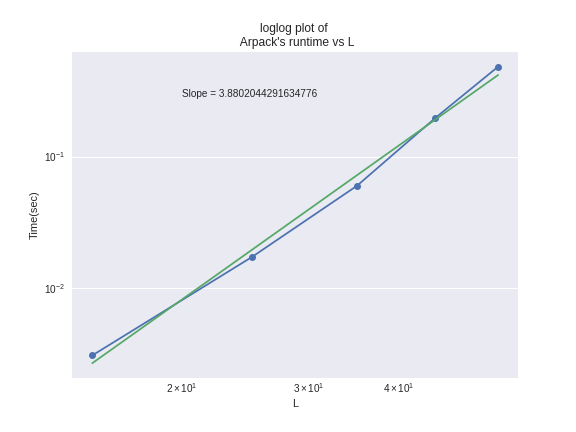
\includegraphics[width=0.45\textwidth]{./images/arpack_loglog.png}
\end{figure}

\begin{figure}[h]
  % \caption{Example of a parametric plot ($\sin (x), \cos(x), x$)}
  \centering
  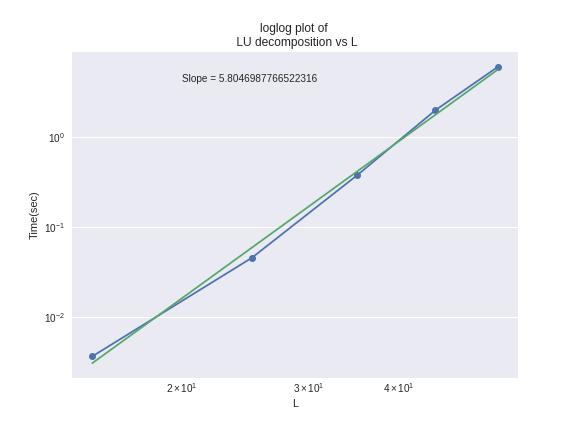
\includegraphics[width=0.45\textwidth]{./images/lu_loglog.png}
\end{figure}

\begin{figure}[h]
  % \caption{Example of a parametric plot ($\sin (x), \cos(x), x$)}
  \centering
  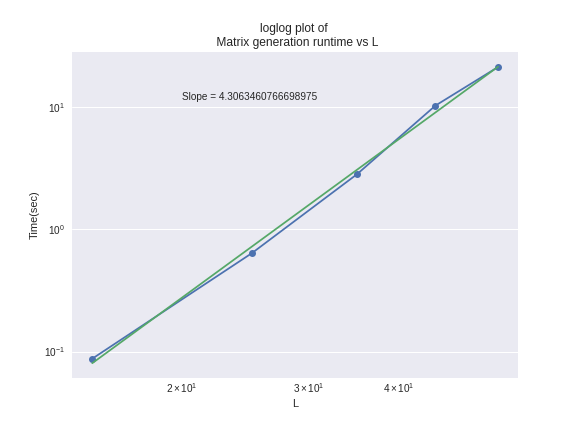
\includegraphics[width=0.45\textwidth]{./images/matrix_generation_loglog.png}
\end{figure}

\begin{figure}[h]
  % \caption{Example of a parametric plot ($\sin (x), \cos(x), x$)}
  \centering
  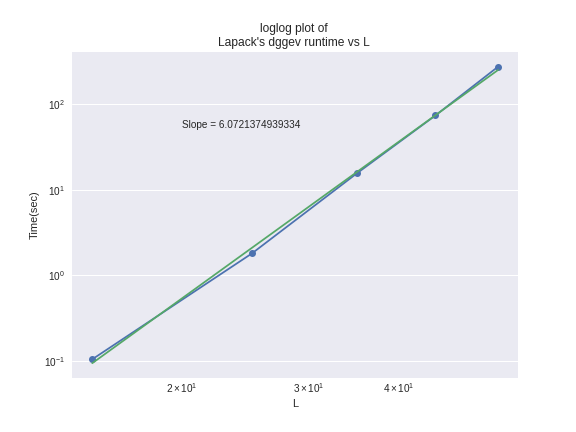
\includegraphics[width=0.45\textwidth]{./images/dggev_loglog.png}
\end{figure}

\subsection{Arpack and Arpack++ guides \label{appen:user_guides}}

Free html version of Arpack guide:
\href{https://www.caam.rice.edu/software/ARPACK/UG/ug.html}{https://www.caam.rice.edu/software/ARPACK/UG/ug.html}

% Free pdf version of Arpack guide:

% \href{http://li.mit.edu/Archive/Activities/Archive/CourseWork/Ju_Li/MITCourses/18.335/Doc/ARPACK/Lehoucq97.pdf}{http://li.mit.edu/Archive/Activities/Archive/CourseWork/Ju_Li/MITCourses/18.335/Doc/ARPACK/Lehoucq97.pdf}


Arpack++ guide:
\href{https://github.com/m-reuter/arpackpp/blob/master/doc/arpackpp.pdf}{https://github.com/m-reuter/arpackpp/blob/master/doc/arpackpp.pdf}


\subsection{For future reference \label{appen:for_future_reference}}


\subsubsection{Possible speedup}

The simplest first possibility that may work is going back to the matrix free version and generating the full matrices every 100th step or so to use as a preconditioner. If the spin does not change very rapidly then the matrix should also change slowly and the same preconditioner could be used for multiple time steps. The main issue is that close to the merger spins will change rapidly, and there we may end up calculate the full matrices at every step defeating the whole purpose. All the following suggestion are simply noting the parts that can be parallelized.


Now that we are using Arpack the bottleneck is matrix generation. The matrix is simply generated by using the action of the matrices on unit vectors. In theory the matrix action function can act on multiple basis vectors in parallel.

After, that the next most costly process is the LU decomposition and using it solve a linear system which is being done by Lapack.

Finally, there is Arpack which takes hardly a few seconds to run once the LU decomposition is done. The chances that we would ever need something faster than it is slim but there is a parallel version of Arpack in the \href{https://github.com/opencollab/arpack-ng/tree/master/PARPACK}{Arpack-ng github repo}.


\subsubsection{Newer versions of Lapack will be faster}
\href{https://github.com/Reference-LAPACK/lapack/pull/421}{A recently merged pull request in Lapack} allows it to solve generalized eigenvalue problems 10-12 times faster. This will still be significantly slower than Arpack for our use case as we are only finding 3 eigenvectors but apparently Lapack can still get faster!


\bibliography{apssamp}% Produces the bibliography via BibTeX.


\end{document}
